\chapter{}
``Quinn, wake up.''

I wasn't deeply asleep, so my mind cleared quickly. The events of the morning replayed in
my mind: Samantha turns out to be an undercover Police officer, the veiled threats and
intimidation attempts from her and the other cop, casting Monique, making love, dozing off
afterward, and now here I was: lying in a tight embrace with Monique, who was naked, save for
the two purple long leg casts she wore. I turned to look at her, and as if I needed reminding,
my bare legs brushed against the rough fiberglass covering her legs.

``Let's go someplace,'' she said, smiling. Damn she was beautiful.

``Where?'' I asked.

``I don't know, let's just get out. I'd like to show off these casts.''

Damn, she's fun, too. She really does like this as much as I do. Maybe even more.

``Sounds good to me.'' I replied. ``You're off work tonight, aren't you?''

``Yes, I don't have to go back in until tomorrow. Let's just get dressed, and have ourselves
a little road trip. We don't even need a destination- let's just drive and see where we end
up,''
she suggested, as she slid out from under the sheet that covered us, and swung her legs to the
side of the bed. ``Could you get me some crutches?''

I went to the casting room and retrieved the jeans and t-shirt Monique had been wearing
before we'd casted her. I also grabbed the aluminum crutches that we'd used on the trip to Cedar
Point. They were already adjusted for Monique's height, and given the events of the last few
days, would probably stay that way. That thought gave me a smile. I started back, then stopped
and also retrieved a pair of cast shoes. They certainly leave a lot to be desired aesthetically,
but they are very convenient.

\begin{thought}
Monique was looking forward to the afternoon ahead. She wasn't sure where they would end
up, or where they would be along the way, but it promised to be a fun adventure. As Quinn
returned, she took a long look at him. He was almost comical looking, standing there naked with
crutches in one hand, and her clothes and cast shoes in the other. Comical or not, the sight of
him filled her with a warmth- the warmth of a woman in love. She knew she loved him. She didn't
know where things would go for them as a couple, but at this point, she was more concerned with
enjoying today than thinking too much about tomorrow.

He laid her clothes on the bed next to her and knelt on the floor at her feet. He started
to strap the cast shoes on her casted feet, then stopped. He looked to the side where her bra
and underwear had landed on the floor where he'd tossed them as he undressed her earlier. He
handed her the bra, and carefully slid the panties over her casted feet to where she could reach
them. He then slid the vinyl cast shoes on, pulled the straps tight, and pressed the Velcro
together. He then grabbed his own clothes and began dressing himself. Monique rocked forward
onto her feet, paused for a moment as she balanced herself, then pulled her underwear the rest
of the way up to her waist. She then leaned back against the bed, and put her bra on.
\end{thought}

I finished dressing myself, and looked at Monique. She was holding up her jeans. ``These are
kind of useless,'' she said. I hadn't thought of that. She rocked forward to her feet again, and
took the crutches, placing one under each arm. She stuck the crutches in front of her, and swung
her legs through. She headed out of the room, and toward the stairs.

``Whoa, just where do you think you're going?'' I asked.

``Upstairs to get dressed,'' she said, as though it were a silly question.

``You're going upstairs- with two long leg casts? Uh-uh. No way. You'll end up hurting
yourself for real. Why don't you tell me what you want, and I'll get it for you?''

\begin{thought}
He was right. A part of her wanted to try; she liked trying to do things for herself almost
as much as she liked being waited on and pampered. This, however, had a real element of danger.
Even if she didn't kill herself trying, it would take forever, and she wanted to get out before
they lost any more daylight.
\end{thought}

She told me to pick out something I liked that fit her situation. I went upstairs and found
some shorts and a tank top. She'd look damn good wearing this with her casts. I went back
downstairs and helped her get dressed. She wanted to clean up a bit and fix her hair, so I
watched her crutch into the downstairs bathroom, and went to load the SUV for the trip.

After tossing the wheelchair, camera and some drawing supplies in the SUV, I heard the back
door open. Monique hobbled out toward the back steps. I headed over to carry her down, but she
waved me off.

``Let me try these, just be ready to catch me if I fall.'' She said.

\begin{thought}
This was only three steps, but unable to bend her legs, it seemed to be an almost
impossible task. Quinn was there, but she wanted to try this. She handed the crutches down to
Quinn, and leaned against the handrail. She held herself with her arms and led with her right
leg. She leaned right against the rail until she was low enough to put her weight on the right
leg, and swing the left one forward. She went down one step at a time, and was pleased with
herself when she reached the bottom. She'd figured it out. Next time, she'd treat herself to
allowing Quinn to carry her.
\end{thought}

I smiled, and shook my head. ``You just HAD to find a way, didn't you?''

She reached out for her crutches and said ``Yes, I wanted to try. I love letting you do
everything for me, but like trying to do things for myself, too. I'll probably need help getting
in the truck, though.''

I followed her to the passenger's side door of the Expedition. I'd moved the seat all the
way back, hoping it would be enough room for her legs. I opened the door, took her crutches and
laid them on the ground. I picked her up and gently placed her in the truck, feet first.
Luckily, there was enough room. I handed her the seat belt, shut the door, and loaded the
crutches in back before getting in, myself.

As we headed down the road, she asked ``So, where are we headed?''

``I don't know, where would you like to head?''

``I don't know, either. Let's just pick a direction, and go until we see something that
catches our interest,'' she said.

It sounded good to me. ``Okay, let's go fill the tank, and then we'll flip a coin to
decide.''

``Sounds good,'' she said. ``But let's make one rule- no interstates. Only country roads.''

``It's a deal,'' I replied as I turned in to the gas station.

The gas station was actually a truck stop near the interstate. I swiped my card, and
started filling the tank when the door opened, and Monique slid out. She hobbled to the back
door, steadying herself with a hand on the side of the truck. She got the crutches, and used
them to get around to the driver's side, where I was.

``I'll be back, I'm going to the restroom,'' She said as she turned toward the building.

``Do you need help?'' I asked.

``No, I'm a big girl- I can go all by myself,'' she said with a smile as she headed away.

\begin{thought}
As she crutched her way into the building, Monique noticed people looking at her. She was
used to getting looks from men, but she seemed to catch everyone's attention now, if only for a
few seconds before they averted their eyes. As she headed past the soda fountain, she noticed a
middle-aged man in a work uniform filling a huge travel cup. The name patch on his shirt read
``Paul.'' Paul was not making any attempt to disguise the fact that he was looking. In fact, she
had his attention so completely that he kept filling his cup until it overflowed! The cold
Mountain Dew pouring over his hand seemed to bring him back to reality as she moved past.

She smiled to herself, and wondered if that man might be a caster. He was certainly
oblivious to the rest of the world as she hobbled past. She chuckled as she thought ``It's a
good
thing he wasn't lighting a cigarette!''
\end{thought}

I finished filling the tank, and took my receipt from the pump. I looked toward the door,
and Monique was headed my way. I noticed a man standing by a delivery truck with ``Cardinal
Kitchens'' painted on the side. The man was watching her intently as she made her way back
toward
me. After she passed, the man took out a cell phone and opened it. I can't be sure, but by the
way he held it, I'm convinced he was taking her picture.

``Thirsty?'' she asked, as she pulled a bottle of Diet Coke from her front pocket and handed
it to me.

``Yes. Thanks.'' I opened the door for her, and took her crutches, and helped her into the
truck. I put the crutches in the back seat, and walked around and slid into the driver's seat.

I pointed in the direction of the man by the delivery truck. ``I think you have a fan,'' I
said with a smile.

She looked his way, and said ``He was sure watching me inside. He poured Mountain Dew all
over his hand,'' she chuckled. ``Maybe he's a caster.''

``Maybe he is. Then again, as beautiful as you are, you're going to get attention anyway.''

``Thank you, dear.'' She said, and leaned over and kissed me. She then took another bottle of
Diet Coke from her other shorts pocket, and unscrewed the lid. She also brought out a quarter,
and said ``Okay. Heads we go east, tails we go west.''

George showed his face to us, and we headed East. Soon we were out of the city, heading
past farms and woods on the country roads. We talked the whole way- we never seemed to run out
of things to talk about: music, travel, books, her schooling, and of course, casting. We talked
about different casts she had worn, and some she wanted to wear. We talked about what she liked
about each one, and which were her favorites. She definitely liked the big casts, and the
cumbersome combinations.

After a couple of hours, we found ourselves in Lexington. We knew we were going in that
direction, but we had no idea we'd end up there until we were actually there. Driving through
town, we saw a mall.

``Quinn, let's go in. Let's walk around for a while.'' I agreed, and pulled in and found a
parking place. I got the wheelchair out of the back, and suggested that I walk, and that she
ride. I helped her into the chair, adjusted the leg rests under her casted legs, and wheeled her
toward the door.

\begin{thought}
Monique was getting an idea. She wondered if Quinn would think it was silly, but to her, it
sounded like a lot of fun. It would throw a serious element of uncertainty and spontaneity into
their cast adventures. She thought over in her mind exactly how to make it work, as well as how
to breach the subject with Quinn.
\end{thought}

As we walked along, I noticed Monique seemed rapt in thought. I wondered if she even was
aware of the attention she was getting from the other shoppers at the mall.

``Hey- penny for your thoughts. You seem a million miles away.''

``Sorry,'' she said. ``I was thinking of putting a new twist into our… playtime.''

``Oh? Care to share? I asked, unsure of what to expect next.

``Well, I need to figure out exactly how to make it work, first. I think it will be…..'' The
answer must have come to her then, because she added ``Yes! That will work great!''

As we walked along, I Asked her ``When are you going to share with me what you're up to?''

``Soon.'' She said with her playful smile. ``I need to figure out a couple more things, but I
think you're going to like this.''

I shook my head in feigned disgust. ``Okay- you'll tell me when you're ready.'' I wheeled her
outside, and decided that I wanted to do a sketch of her in the wheelchair.

``Do you mind if I draw while you think?

``Not a bit,'' she answered. I started toward the truck to get my pad and pencil and told her
I'd be right back.

\begin{thought}
``I hope he likes this idea,'' Monique thought to herself as she waited for him to return.
She remembered a plotline of a casting story she'd read online, and how what had happened in the
story had seemed like a lot of fun to her, even if the woman in the story hadn't found it very
enjoyable. She smiled at Quinn as he returned to her, sat down, and began drawing. As he worked,
she thought through the numbers in her head. She'd need a pencil and paper to finalize things,
but the plan, and how it would work was taking shape in her head. She watched Quinn work over
the paper, and found herself just getting lost in his gaze. Her heart felt fulfilled in a way it
never had before. She knew this was truly special.
\end{thought}

I showed her the finished drawing. She mentioned how she loved the way I captured her with
my pencil. She wanted to head home, so we headed out to the truck, loaded up and were on our
way. My curiosity was getting the best of me, so I asked her ``When do I get let in on this
great
idea of yours.''

``Every time we cast, one of us makes a suggestion, and then we talk about it, and sometimes
we take a lot of time deciding things. What if we took the deciding out of it?''

``How?''

``Totally randomly.'' She said with a smile.

\begin{center}
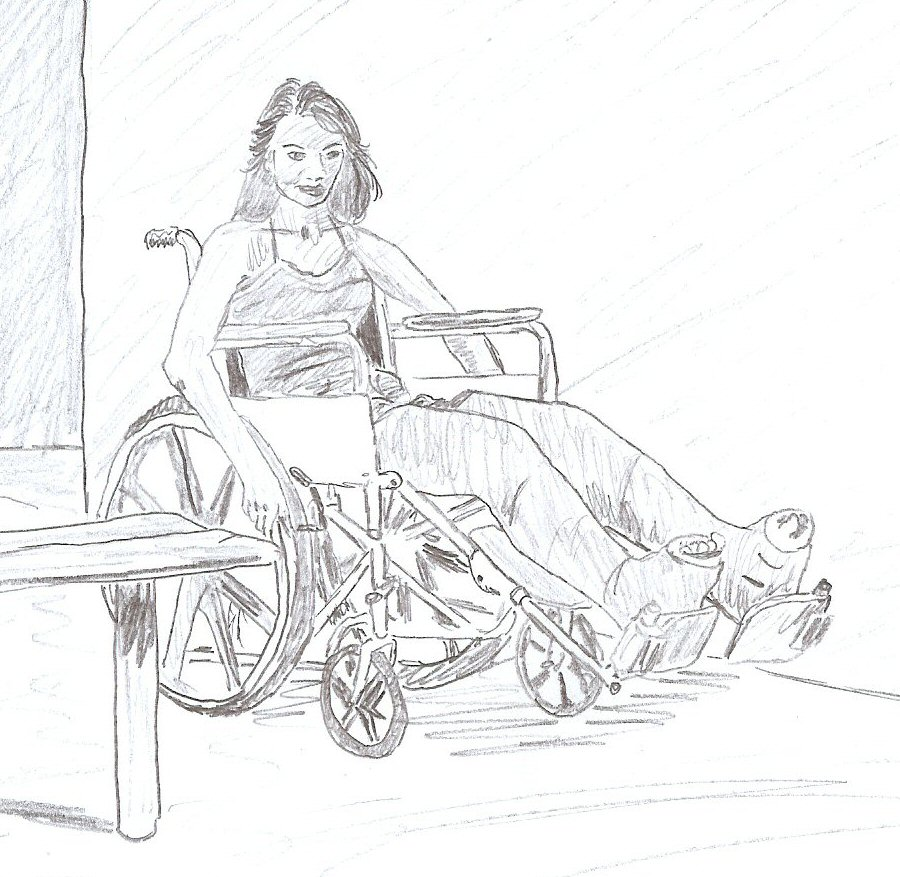
\includegraphics{images/kicks35.jpg}
\end{center}
